%Statistics gathered during operation.
%Graphs, numbers, etc. Explain your results! What
%do your measurements show/mean?
\section{Statistics}

\begin{wrapfigure}{r}{0.6\textwidth}
  \vspace{-30pt}
  \begin{center}
    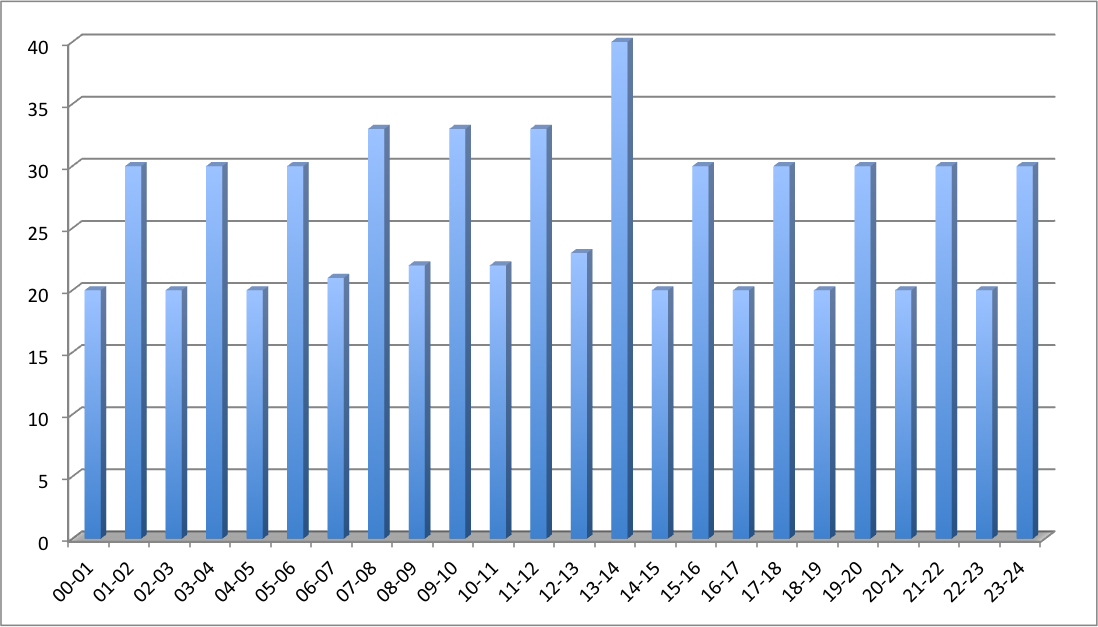
\includegraphics[scale=0.5]{img/per-hour.png}
  \end{center}
  \vspace{-20pt}
  \caption{\bf{Email per hour of each day}}
  \hspace*{20pt}
\end{wrapfigure}

We have also monitored the operation through statistics generated by Exim. The period we monitored spanned from the 7th of March through to the 16th.\newline

%\begin{wrapfigure}{l}{0.7\textwidth}
  %\vspace{-20pt}
  %\vspace{-20pt}
  %\caption{\bf{Rejection reasons}}
%\end{wrapfigure}

The first table (fig. 1) describes the amount of email processed (sent and received) during the different hours of the days. This is highly relevant in order to pick a good time for maintenance. However, as is visible from the table, a email server that is always active is difficult to maintain without interrupting the users.\newline

\begin{figure}[htb]
  \begin{center}
    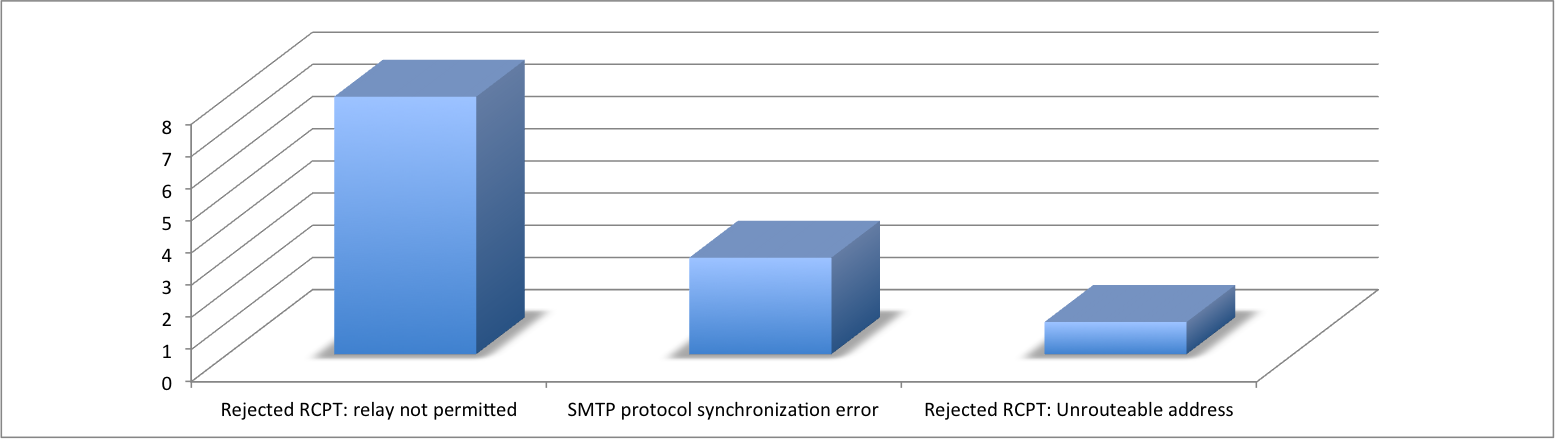
\includegraphics[scale=0.55]{img/rejection-reasons.png}
  \end{center}
  \caption{\bf{Reasons for rejection}}
\end{figure}

As an operator it's interesting to know why a particular email did not reach it's destination. The second table (fig. 2) describes the different reasons for rejection and lists how many individual emails were affected.\newline

\begin{figure}[h!]
%  \vspace{-20pt}
  \begin{center}
    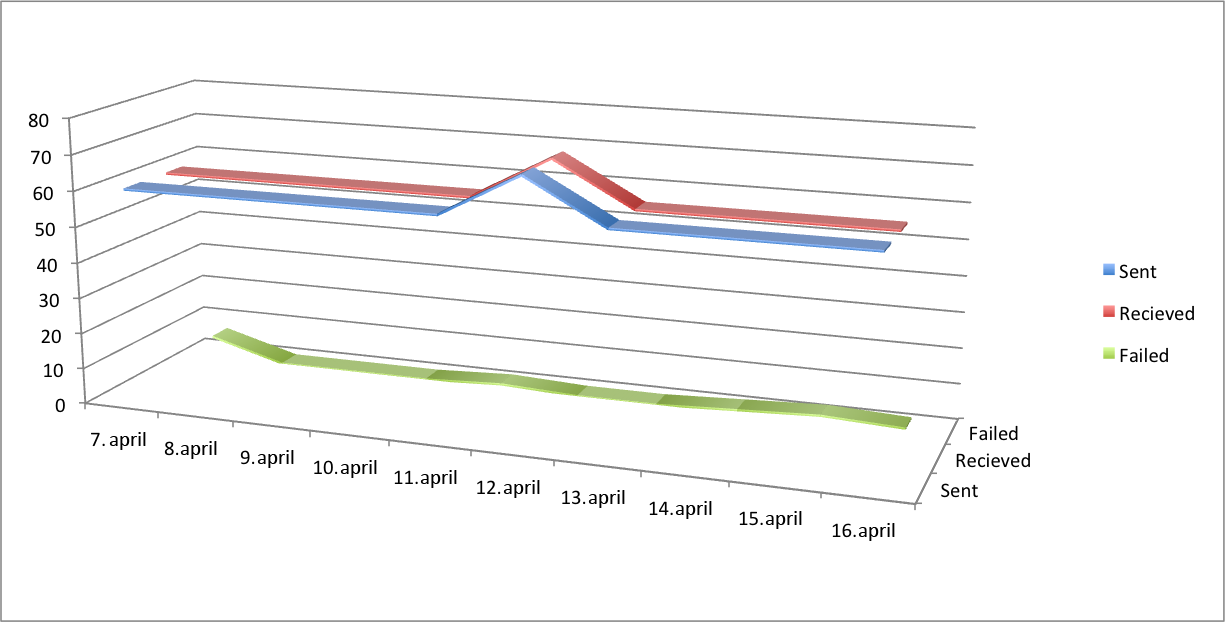
\includegraphics[scale=0.70]{img/sent-received-failed.png}
  \end{center}
 % \vspace{-20pt}
  \caption{\bf{Amount of email per day}}
\end{figure}

The last table (fig. 3) describes the amount of email per day. From the straight and coherent lines showing the sent and received statistics we can deduct that all mail was probably sent and received by the same server, i.e. the users of this particular email system were only contacting eachother. The error rate is stable and fairly close to zero.\newline